\documentclass[14pt,aspectratio=169]{beamer}

\usepackage[russian]{babel}
\usepackage{amsmath}
\usepackage{amsfonts}
\usepackage{graphicx}
\usepackage{amsthm}
\usepackage{fontspec}

\setmainfont{Times New Roman}
\setsansfont{Times New Roman}

\usetheme{Madrid}
\usecolortheme{default}

\theoremstyle{definition}
\newtheorem{defn}{Определение}

\title{Абсолютная устойчивость}
\subtitle{Проблема Лурье и критерии устойчивости}
\author{Зыкин Л. В., Алехова М. С., Кисиков Д. С.}
\institute{Университет ИТМО \\ Факультет систем управления и робототехники}
\date{2025}

\begin{document}

\frame{\titlepage}

\begin{frame}
\frametitle{Содержание}
\tableofcontents
\end{frame}

\section{Введение}

\begin{frame}
\frametitle{Проблема абсолютной устойчивости}
\begin{itemize}
    \item \textbf{Задача}: гарантировать устойчивость системы с \emph{неопределённой} нелинейностью
    \item \textbf{Идея}: задать класс допустимых нелинейностей и обеспечить устойчивость для \textbf{всех} функций из этого класса
    \item \textbf{История}:
    \begin{itemize}
        \item 1944: А. И. Лурье сформулировал проблему
        \item 1957: В. М. Попов предложил частотный критерий
        \item 1960-е: Р. Калман и В. А. Якубович — лемма КЯП
    \end{itemize}
\end{itemize}

\vspace{10pt}
\textbf{Применение}: системы с насыщением, реле, адаптивные системы, робастное управление
\end{frame}

\begin{frame}
\frametitle{Основные понятия}
\begin{defn}[Абсолютная устойчивость]
Система называется \textbf{абсолютно устойчивой} в классе нелинейностей $\Phi$, если:
\begin{enumerate}
    \item Нулевое решение $x=0$ глобально асимптотически устойчиво
    \item Для \emph{всех} функций $\varphi\in\Phi$ и любых начальных условий
    \item Решение $x(t)\to 0$ при $t\to\infty$
\end{enumerate}
\end{defn}

\vspace{10pt}
\textbf{Ключевая особенность}: робастность по отношению к неопределённости в описании нелинейного элемента
\end{frame}

\section{Постановка задачи}

\begin{frame}
\frametitle{Форма Лурье}
Рассматривается SISO-система:
\begin{equation*}
    \begin{aligned}
        \dot x &= Ax + b\,\varphi(\sigma),\\
        \sigma &= c^\top x, \qquad y = \sigma,
    \end{aligned}
\end{equation*}
где:
\begin{itemize}
    \item $x\in\mathbb{R}^n$ — вектор состояния
    \item $A\in\mathbb{R}^{n\times n}$ — матрица линейной части (гурвицева)
    \item $b, c\in\mathbb{R}^n$ — векторы входа и выхода
    \item $\varphi:\mathbb{R}\to\mathbb{R}$ — статическая нелинейность
\end{itemize}

\vspace{10pt}
Передаточная функция линейной части:
\begin{equation*}
    G(s) = c^\top (sI - A)^{-1} b
\end{equation*}
\end{frame}

\section{Классы нелинейностей}

\begin{frame}
\frametitle{Секторные ограничения}
\begin{defn}[Сектор $[k_1, k_2]$]
Функция $\varphi:\mathbb{R}\to\mathbb{R}$ принадлежит сектору $[k_1, k_2]$, если:
\begin{equation*}
    k_1\sigma^2 \le \varphi(\sigma)\sigma \le k_2\sigma^2, \quad \forall \sigma\in\mathbb{R}, \quad \varphi(0)=0
\end{equation*}
\end{defn}

\vspace{10pt}
\textbf{Геометрически}: график $\varphi(\sigma)$ лежит между прямыми $y=k_1\sigma$ и $y=k_2\sigma$

\vspace{10pt}
\textbf{Примеры}:
\begin{itemize}
    \item Насыщение: $\varphi(\sigma) = \mathrm{sat}(\sigma)$ — сектор $[0,1]$
    \item Реле: $\varphi(\sigma) = k\,\mathrm{sign}(\sigma)$ — сектор $[0,k]$
\end{itemize}
\end{frame}

\section{Критерии абсолютной устойчивости}

\begin{frame}
\frametitle{Круговой критерий}
\begin{theorem}[Круговой критерий]
Система абсолютно устойчива в секторе $[0, k]$, если:
\begin{enumerate}
    \item Матрица $A$ гурвицева
    \item Найквист-диаграмма $G(j\omega)$ не охватывает точку $(-1/k, 0)$
    \item Эквивалентно: $\Re\{G(j\omega)\} > -1/k$ для всех $\omega$
\end{enumerate}
\end{theorem}

\vspace{10pt}
\textbf{Геометрическая интерпретация}: кривая Найквиста целиком правее вертикальной прямой $x = -1/k$
\end{frame}

\begin{frame}
\frametitle{Критерий Попова}
\begin{theorem}[Критерий Попова]
Система абсолютно устойчива в секторе $[0, k]$, если существует $\nu\ge 0$ такое, что:
\begin{equation*}
    \Re\big\{(1+j\omega\nu) G(j\omega)\big\} > -\frac{1}{k}, \quad \forall \omega\in\mathbb{R}
\end{equation*}
\end{theorem}

\vspace{10pt}
\textbf{Преимущества}:
\begin{itemize}
    \item Менее консервативен, чем круговой критерий
    \item Параметр $\nu$ позволяет учитывать фазовые свойства
    \item Модифицированная Найквист-диаграмма $(1+j\omega\nu)G(j\omega)$ правее прямой $x = -1/k$
\end{itemize}
\end{frame}

\begin{frame}
\frametitle{Лемма Калмана--Якубовича--Попова (LMI)}
\begin{theorem}[LMI-критерий]
Система абсолютно устойчива в секторе $[0, k]$ тогда и только тогда, когда существуют $P=P^\top>0$ и $q\ge 0$ такие, что:
\begin{equation*}
    \begin{bmatrix}
        A^\top P + P A & P b - q c\\
        b^\top P - q c^\top & -2q/k
    \end{bmatrix} < 0
\end{equation*}
\end{theorem}

\vspace{10pt}
\textbf{Преимущества LMI-формулировки}:
\begin{itemize}
    \item Эффективная численная проверка (SDP)
    \item Возможность синтеза регуляторов
    \item Учёт неопределённостей в параметрах
    \item Обобщение на MIMO-системы
\end{itemize}
\end{frame}

\section{Пример}

\begin{frame}
\frametitle{Пример: анализ системы}
\textbf{Линейная часть}: $G(s) = \dfrac{1}{s(s+2)}$

\vspace{10pt}
В пространстве состояний:
\begin{equation*}
    \begin{aligned}
        \dot x_1 &= x_2,\\
        \dot x_2 &= -2x_2 + \varphi(\sigma),\\
        \sigma &= x_1
    \end{aligned}
\end{equation*}

\vspace{10pt}
\textbf{Нелинейность}: сектор $[0, 1]$

\vspace{10pt}
\textbf{Проверка по критерию Попова}: при $\nu = 1{,}2$ условие выполняется для всех $\omega$

\vspace{10pt}
\textbf{Вывод}: система абсолютно устойчива для любых $\varphi\in[0,1]$ (насыщение, реле и т.п.)
\end{frame}

\begin{frame}
\frametitle{Численная иллюстрация}
\begin{columns}
\column{0.5\textwidth}
\centering
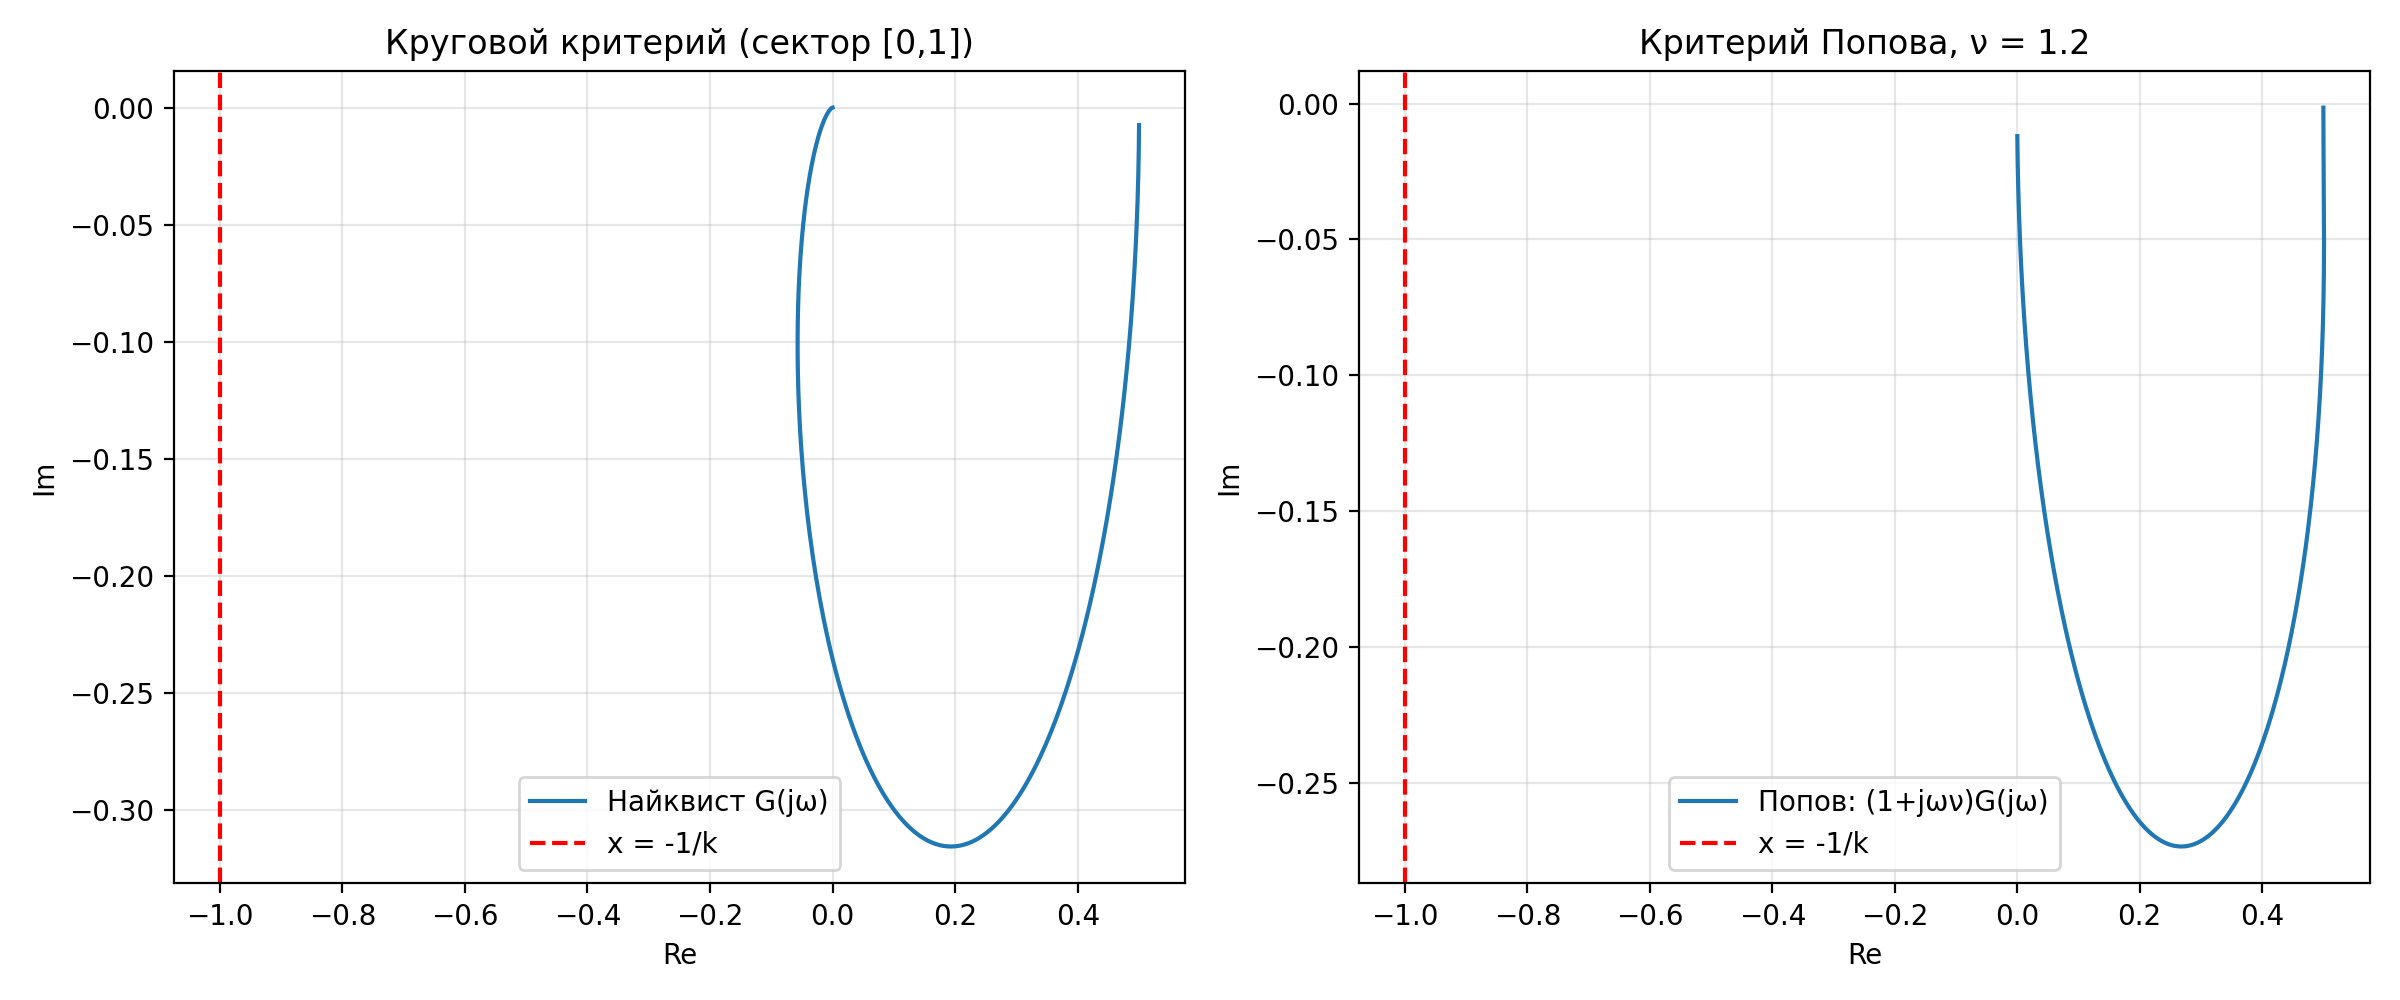
\includegraphics[width=0.9\textwidth]{images/nyquist_popov.png}
\vspace{-5pt}
\small Найквист и кривая Попова

\column{0.5\textwidth}
\centering
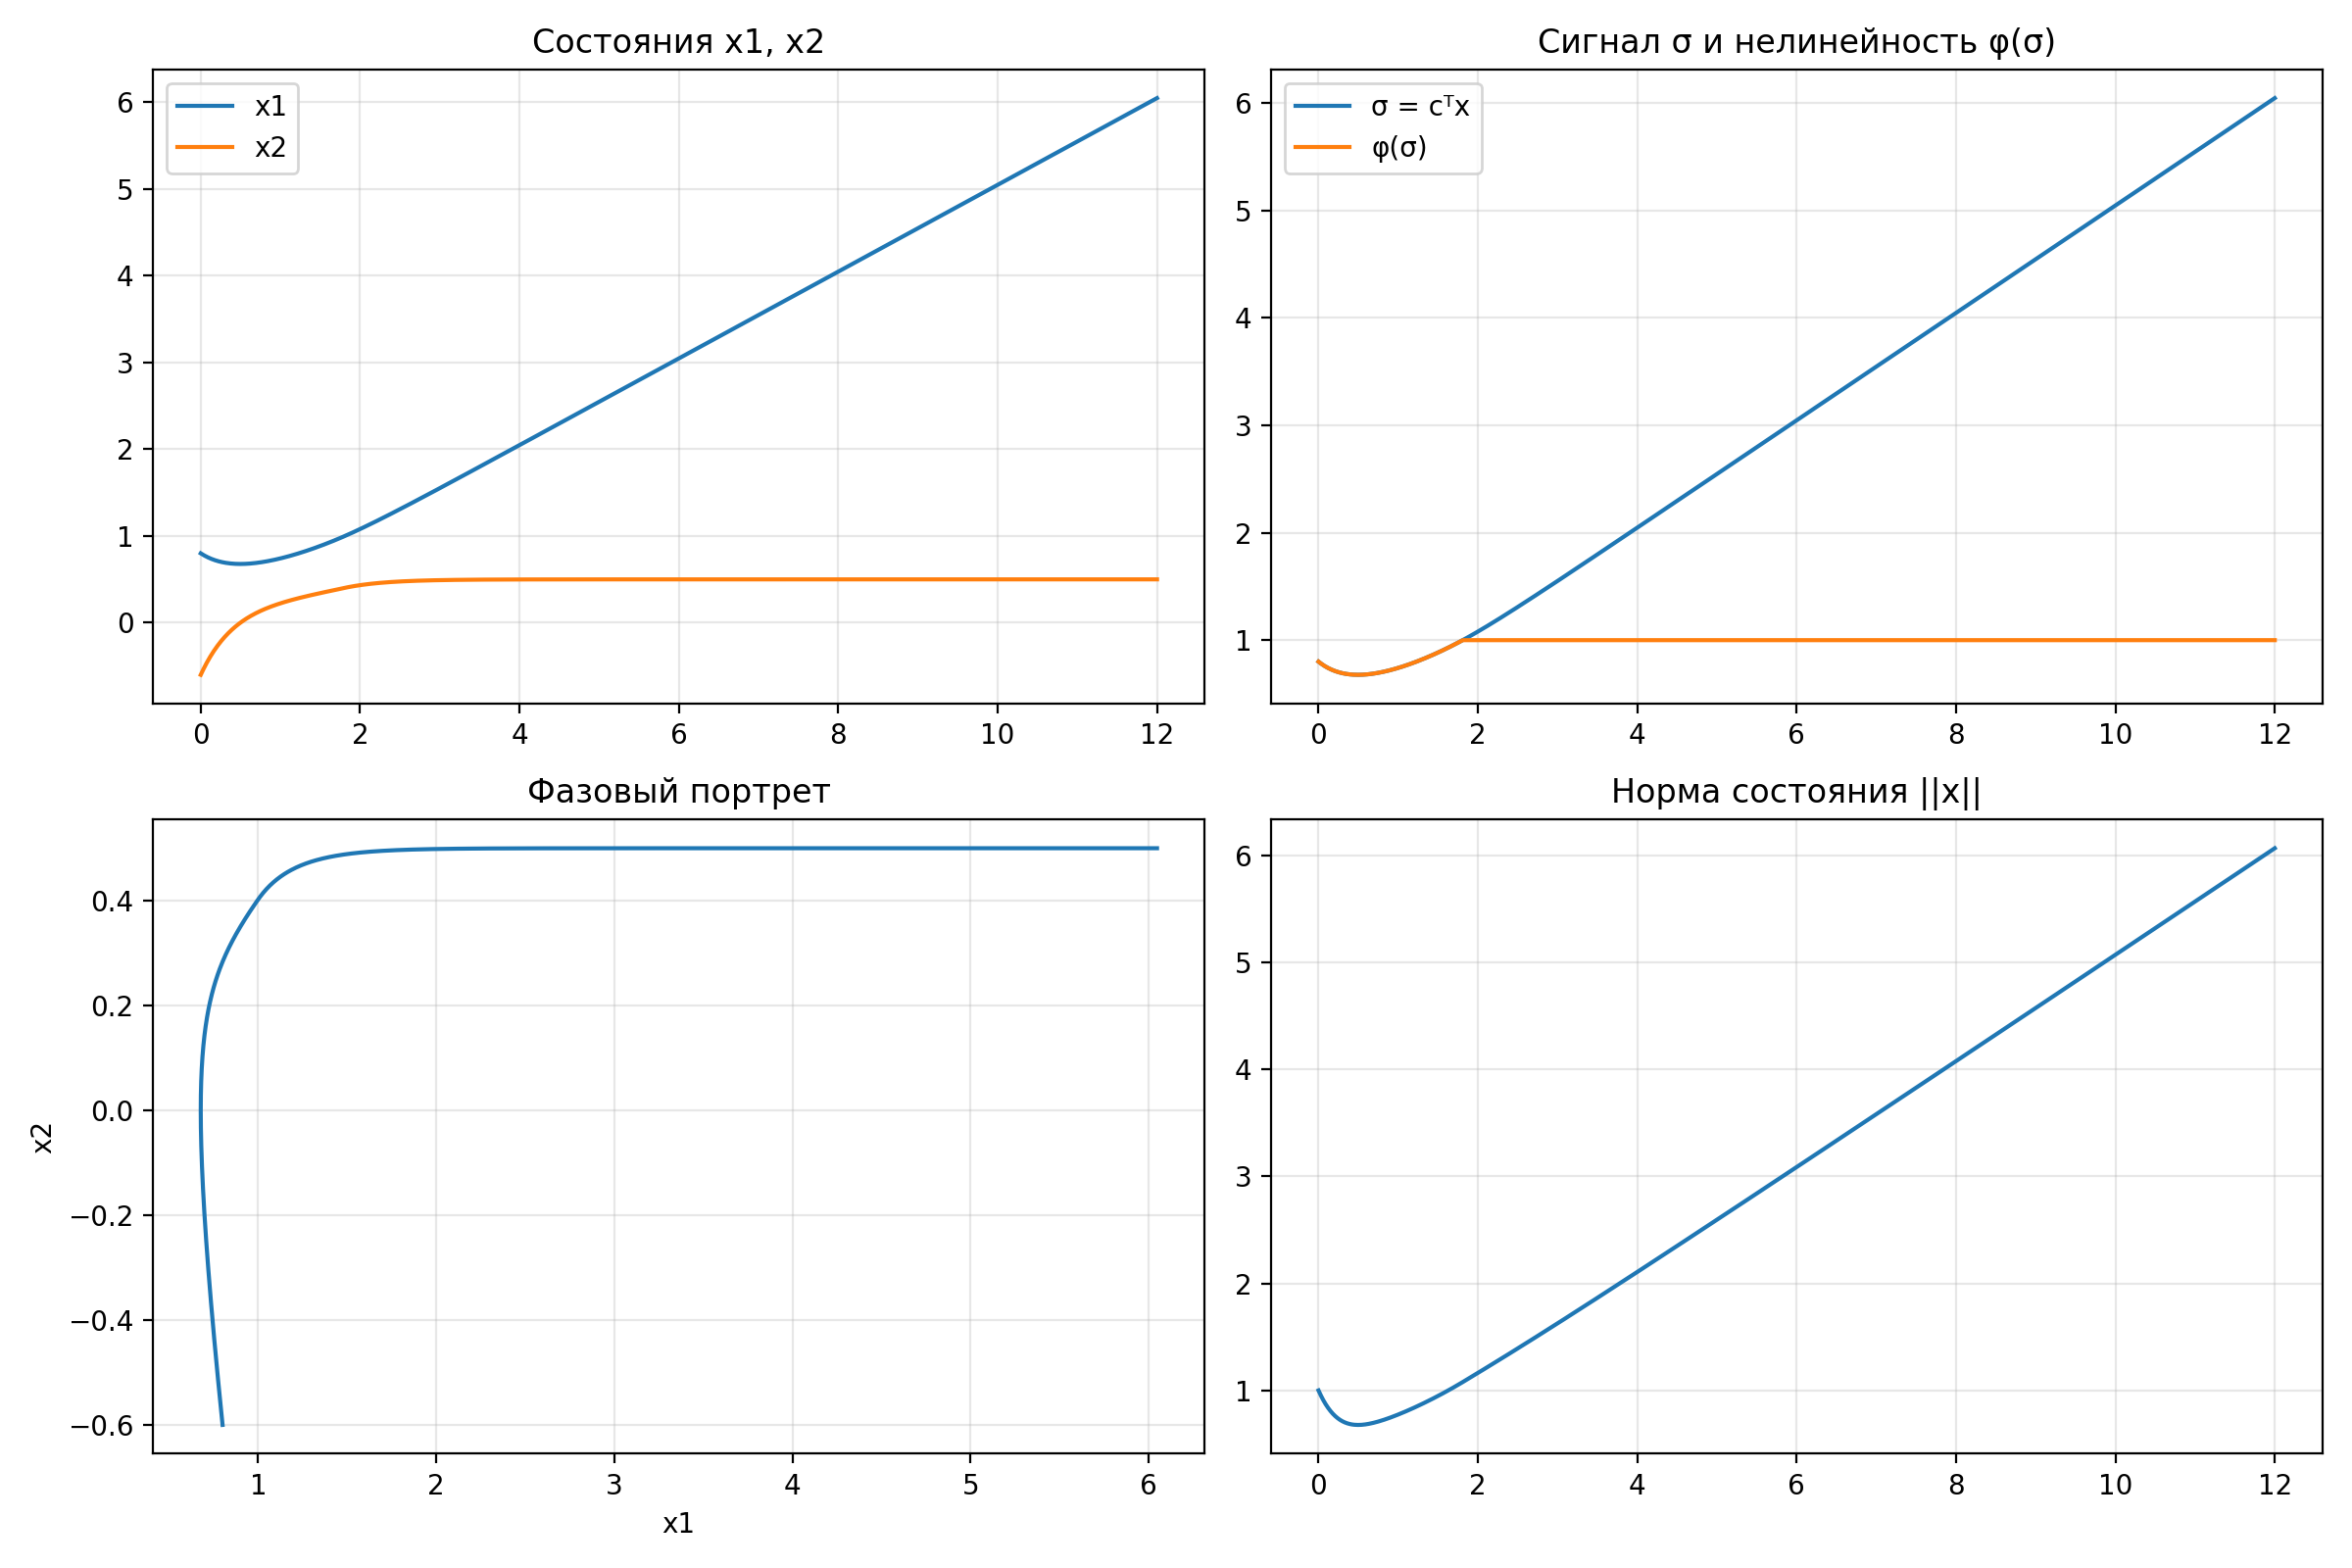
\includegraphics[width=0.9\textwidth]{images/time_response.png}
\vspace{-5pt}
\small Переходный процесс
\end{columns}
\end{frame}

\section{Выводы}

\begin{frame}
\frametitle{Выводы}
\begin{itemize}
    \item \textbf{Робастность}: устойчивость для всего класса нелинейностей без знания их точной формы
    
    \item \textbf{Критерии}:
    \begin{itemize}
        \item Частотные (круговой, Попова) — геометрическая интерпретация
        \item LMI (КЯП) — численная проверка
    \end{itemize}
    
    \item \textbf{Применение}: системы с ограничениями, робастное управление, адаптивные системы
    
    \item \textbf{Ключевой фактор}: корректное определение сектора нелинейности
\end{itemize}
\end{frame}

\begin{frame}
\frametitle{}
\begin{center}
    \Large Спасибо за внимание!
\end{center}
\end{frame}

\end{document}

